% -*- root: ../main.tex -*-
%!TEX root = ../main.tex
% this file is called up by main.tex
% content in this file will be fed into the main document
% vim:textwidth=80 fo=cqt

Having performed a  comprehensive analysis of the state of  the art in \gls{spm}
modelling, this section presents the  author's unique contribution to the field.
Firstly, the  scope of the  contribution is identified. The  methodology adopted
and corresponding results are presented thereafter.

\subsection{Scope and motivation}\label{subsec:scopenewelectrolyte}

This subsection is intended as a capstone summary helping to briefly recount the
discussion so far  and to provide a  context for the author's work  in the wider
realm  of the  \gls{spm}  modelling art.  In  the same  vein  as the  discussion
in~\cref{sec:electrolyteinclusion}, the scope of the proposed enhancement to the
\gls{spm} concerns entirely  with improving the electrolyte subsystem  as it has
already been established in~\cref{subsec:simresultsbasicspm} that the simplified
representation of  the solid-phase subsystem  through a fourth  order polynomial
approximation method  for diffusion of  \ch{Li^0} in  the solid particle,  is of
sufficiently high accuracy.

Inspecting the  electrolyte domain,  the electrolyte  overpotential contribution
to  terminal  voltage   consists  of  a  diffusion   overpotential  in  addition
to   the  time-dependent   ohmic  losses   that  originates   from  differential
concentration  gradients  that  is   indirectly  dependent  upon  concentration.
Hence,  accurate  determination  of   spatio-temporal  concentration  takes  the
centre  stage.  For   the  computation  of  overpotential   in  the  electrolyte
phase,~\cref{eq:electrolytepdwithce}  proposed  by  Prada~\etal~\cite{Prada2012}
may be used.

There exists a  subtle detail in the  use of~\cref{eq:electrolytepdwithce} which
is discussed here upfront before proceeding  ahead to the refined context of the
author's  work.  The  intrinsic  conductivity  of  electrolyte,  $\kappa$  is  a
function of  the ionic concentration  (refer~\cref{subsec:basicspmsimsetup}). If
the ionic  concentration at  the corresponding current  collectors are  used for
$\kappa_\text{neg}$  and  $\kappa_\text{pos}$, this  would  lead  to a  lopsided
computation of the overpotential in electrolyte. Furthermore, under this scheme,
the computation of electrolyte conductivity shall be rendered ambiguous since it
is unclear which  separator interface shall be chosen for  the separator's ionic
concentration. Although this  has not been discussed clearly  in literature, the
author  of this  thesis chose  to use  the mean  concentration within  each cell
region, defined as
\begin{equation}
    \mean{c}_{\text{e},j}(t) = \frac{1}{l_j}\int_0^{l_j} c_{\text{e}_j}(z,t)\, dz = \frac{Q_{\text{e,}j}(t)}{\varepsilon_j l_j}
\end{equation}
although other measures  of central tendency might be equally  valid. Hence, the
results of this section have the associated variability in them depending on how
the electrolyte concentration computations are  used in evaluating the intrinsic
conductivity of electrolyte.

As  the  ionic  concentration  has  both  a  direct  and  indirect  contribution
in~\cref{eq:electrolytepdwithce}, its spatio-temporal  computation is a critical
aspect. As discussed  in~\cref{sec:quadraticapprox}, the quadratic approximation
is a widely used spatio-temporal model for electrolyte concentration which makes
the best  use of available physical  constraints. As established in  the results
of~\cref{subsec:quadraticsimresultsanalysis}, while  the spatial  performance of
the quadratic approximation approach is acceptable, its time-domain performance,
particularly at the crucial current collector locations is mediocre at best.

Thus,   the  \emph{scope}   of  the   author's  work   is  to   obtain  suitable
alternate   expressions   for   improving  the   computation   of   \textbf{time
evolution}  of  the electrolyte  concentration  whilst  retaining the  quadratic
approximation   approach   for  describing   its   spatial   profile.  Such   an
approach  is motivated  by  the  keen observation  that  the baseline  quadratic
approximation  model  has  a  natural  `pause'  in  its  model  description.  To
clarify,~\crefrange{eq:cecontinuitynegsep}{eq:Qepbyintegration}  form a  tightly
coupled set of  seven linear equations in seven unknowns.  The time evolution of
$Q_{\text{e,}j}$  are described  through  a system  of  first order  \glspl{ode}
given by~\crefrange{eq:negliionmolesquadratic}{eq:posliionmolesquadratic}.  In a
practical  implementation,  these  \glspl{ode}  are solved  independently  in  a
decoupled  manner,\ie{}  by using  the  coefficients  obtained from  the  linear
system of~\crefrange{eq:cecontinuitynegsep}{eq:Qepbyintegration} in the previous
time-step. The  author's hypothesis is that  by taking advantage of  the natural
break  in the  operational  sequence which  involves  two separate  computations
between  two independent  subsystems (for  all practical  purposes), it  must be
possible  to  replace  the  underperforming time-evolution  equations  from  the
baseline quadratic approximation with a superior alternate model.

\subsection{Methodology --- System identification} % might have to change section title if TF-based identification becomes a full-fledged subsection

This section presents the methodology adopted in obtaining an improved model for
the rate of evolution  of overall moles per unit area of  \ch{Li^+} ions in each
of the three regions of the cell.

\subsubsection*{Background}\label{subsubsec:sysidbackground}

This  section presents  the  background and  thought  process in  systematically
arriving  at  the  choice of  the  methodology  that  was  adopted for  the  new
time-evolution model of the electrolyte concentration.

Based  upon the  experience  gained  in dealing  with  the literature  presented
in~\cref{sec:electrolyteinclusion}, it is  the author's view that,  owing to the
complex behaviour of electrolyte, a  naive top-down approach \ie{} including all
the physics upfront  followed by a systematic simplification, might  result in a
model that is  mathematically intractable for adoption in  an embedded \gls{bms}
environment.  The baseline  quadratic  approximation method  has  proven that  a
bottom-up  approach, \ie{}  pre-assuming a  simplified structure  for the  final
model  and adapting  its coefficients  to physical  constraints yields  a viable
candidate for inclusion in the conventional \gls{spm}.

Upon  a   closer  examination   of  the  rubrics   of  the   baseline  quadratic
approximation  model, it  comes  to  light that  the  natural `pause'  discussed
towards  the  end  of~\cref{subsec:scopenewelectrolyte}  permeates  to  a  level
more  than  merely  having  to  operate  sequentially  on  two  pseudo-decoupled
subsystems  --- it  goes to  the extent  of rendering  the operating  philosophy
of  fitting  physical  equations  semi-void.   To  clarify  this  statement  and
to  substantiate   the  claim,  while  there   is  no  doubt  that   the  linear
algebraic   equations  of~\crefrange{eq:cecontinuitynegsep}{eq:Qepbyintegration}
do    incorporate    physical    principles   from    the    \gls{dfn}    model,
the     same     does     not      hold     true     for     the     \glspl{ode}
of~\crefrange{eq:negliionmolesquadratic}{eq:posliionmolesquadratic}.   In  fact,
all   the   boundary   conditions   from   the   \gls{dfn}   model   have   been
exhausted   by  this   stage  (refer~\cref{subsec:quadraticsimresultsanalysis}).
Although~\crefrange{eq:negliionmolesgen}{eq:posliionmolesgen}     are    derived
from     the      \gls{dfn}     model,      the     coefficients      of     the
diffusivities   in    the   \gls{rhs}   of    the   next   set    of   equations
\ie{}~\crefrange{eq:negliionmolesquadratic}{eq:posliionmolesquadratic},   merely
involve  substitutions  of the  spatial  derivatives  of the  assumed  quadratic
expression.

Herein lies the weakness of the  baseline quadratic approach. Unlike the spatial
algebraic equations, which are tightly bound by the continuity and flux boundary
conditions at the  separator interfaces, there is no equality  constraint on the
spatial  derivative, which  is free  to grow  or shrink  without any  explicitly
imposed  bounds.  The  onus  of  being accurate  is  therefore  on  the  spatial
derivative evaluation which in-turn depends  on the correctness of the quadratic
functions~(\crefrange{eq:cenquadreduced}{eq:cepquadreduced})  themselves. It  is
not feasible to quantify the magnitude of error introduced in the time-evolution
of concentration  given a small-signal  perturbation in the coefficients  of the
quadratic spatial  computation,\ie{} the implicit  coupling between them  is not
transparent. Since the quadratic approximation itself is not perfect, \ie{} does
not capture the  spatial gradient \emph{exactly} as the \gls{p2d}  model as seen
in~\cref{fig:spatialionicconc1C}, the internal coupling of coefficients leads to
errors in time-evolution computation.

The author's  approach is to  therefore break this detrimental  coupling between
spatial  derivative of  concentration  and its  temporal evolution  counterpart.
Inspired by the fact that the  quadratic approximation model had almost achieved
the desired goals with
\begin{enumerate}[label=\emph{\alph*})]
    \item a bottoms-up approach, \ie{} assuming some model structure apriori, and
    \item not bound by any physical considerations due to the exhaustion of governing equations
\end{enumerate}
have led  the author  to broach  a modelling concept  that exhibit  these common
traits,  yet  of  a  completely  different nature  and  hitherto  unexplored  in
physics-based  battery  modelling  in   general  and  electrolyte  modelling  in
particular --- \emph{black-box system identification}.

\subsubsection*{Brief introduction to system identification}\label{subsubsec:introsysid}

An in-depth  coverage of the topic  of system identification is  well beyond the
scope of  this thesis.  However, keeping  in mind the  interests of  the battery
modelling community  who might not be  familiar with this subject  area, a brief
overview of the core ideas that  are essential for tackling the specific problem
at hand, is presented. For readers  further interested in this topic, the author
suggests the textbook by  Ljung~\cite{Ljung1999} for a comprehensive theoretical
treatment of the foundation topics in system identification.

System identification aims  to provide a mathematical model  of the input-output
mapping  of  a system\footnote{The  precise  definition  of what  constitutes  a
`system' is detailed  in Ljung's textbook. However, for  all practical purposes,
in this  thesis the word `system'  stands for any unknown  entity whose terminal
behavioural model  is being  sought for ---  primarily from  input-output data.}
under consideration. The three categories of system identification are:


\begin{enumdescriptnum}[leftmargin=!,itemsep=1ex,labelwidth=\widthof{$\symbf{\text{brugg}_j}\ \scriptstyle (\times 3)$abc}
    ,partopsep=0pt
    ,topsep=0pt
    ]

\item[White box] wherein underlying physical equations are completely known. The
numerical value  of coefficients of  governing equations are to  be parametrised
from input-output data.

\item[Black box]  wherein no  governing equations are  available for  the system
under  consideration. The  model formulation  is facilitated  by a  rich set  of
system theory  which proceeds by exciting  the system with input  waveforms with
certain desirable  properties and correlating characteristics  from the response
in order  to draw  conclusions about viable  mathematical structures  capable of
emulating  the  terminal  behaviour  of the  system  under  generalised  inputs.
Black  box system  identification was  employed for  the specific  problem under
consideration and hence all future descriptions will pertain to this class.

\item[Grey box] is a hybrid of the  two approaches wherein a part of the model's
governing  physics is  known a  priori, \eg{}  the structure  of a  well-defined
subsystem  that is  part  of a  large,  complex  system may  be  known ahead  of
time,  where the  task  is  to characterise  the  full  system. Grey-box  system
identification tasks can  often be reduced to a single  sub-problem of black-box
system  identification  by  removal  of  the known  physics  and  tackling  them
separately.

\end{enumdescriptnum}

\subsubsection*{Overview of black-box system identification}\label{subsubsec:introblackboxsysid}
Black-box system identification techniques can be broadly classified into ---
\begin{enumerate*}[label=\emph{\alph*})]
     \item non-parametric methods, and
     \item parametric methods.
 \end{enumerate*}

Non-parametric methods do not seek  a pre-assumed mathematical structure for the
system. They  aim to  directly estimate  the very  kernel of  what characterises
every system \viz{}  the Markov parameters in the time-domain  and the \gls{frf}
in the frequency domain, thereby requiring \emph{infinite} number of data points
for  their representation.  Major non-parametric  system identification  methods
include:
\begin{itemize}[topsep=0pt]
    \item Identification in time domain
        \begin{itemize}

            \item Direct  estimation of the system's  Markov parameters through
                statistical correlation of its response to an unit-pulse input

        \end{itemize}
    \item Identification in frequency domain,  \ie{} of the \gls{frf}
        \begin{enumerate}

            \item   Direct   estimation    through   input-output   statistical
                cross-correlation

            \item  \gls{etfe} using \glspl{dft} of input and output sequences

            \item  Smoothed periodogram estimates using Welch's method

            \item  Blackman-Tukey  estimation   method  using  standard  filter
                windows  in digital  signal processing  (such as  Hamming, Hanning,
                Bartlett, Boxcar etc.)

        \end{enumerate}
\end{itemize}

Parametric  methods  aim  to  fit  specific input-output  data  to  some  family
of  well-known  mathematical  constructs  that  generalise  well  to  a  variety
of  inputs.  It  is  important  to recognise  that,  in  contrast  to  white-box
system identification, the salient coefficients/properties of these mathematical
structures do  not, in any way  correspond to physical properties  of the system
under consideration. Major parametric system identification methods are:
\begin{itemize}
    \item Transfer-function based frequency domain model structures
        \begin{enumerate}
            \item \gls{oe} model
            \item \gls{arx} model
            \item \gls{armax} model
            \item Box-Jenkins (BJ) model
        \end{enumerate}
    \item State-space time-domain model structures
        \begin{enumerate}
            \item Ho-Kalman realisation
            \item \gls{era} realisation
            \item Deterministic and stochastic \emph{subspace} structures
        \end{enumerate}
\end{itemize}

Among  these  system  identification  methods, the  non-parametric  methods  are
immediately  ruled  out   for  applying  to  the  task  at   hand.  As  outlined
in~\cref{subsubsec:sysidbackground},  the author  is  inspired by  the trait  of
having  a  pre-assumed  model  structure that  brought  the  baseline  quadratic
approximation closer to a successful  realisation. The non-parametric methods do
not conform to this philosophy.  Furthermore, the requirement of infinite number
of data  samples in order to  fully quantify the system  dampens its feasibility
for implementation  in resource constrained  environments. The author is  of the
opinion that resorting  to truncation of the characteristic  sequence shall only
yield a sub-optimal solution.

While  parametric state-space  identification is  a feasible  alternative, these
methodologies  are   tedious  and   error-prone.  For  instance,   applying  the
Ho-Kalman  algorithm requires  construction  of  Block-Hankel matrices  followed
by  a  \gls{svd} operation.  The  \gls{era}  brings  with  an identical  set  of
operations  of  the  Ho-Kalman  procedure, except  that  certain  random  blocks
in  the  Hankel   matrices  are  chosen  at  random  for   deletion  for  better
estimates  in  low \gls{snr}  environments  and  for capturing  slowly  decaying
phenomena  with long  time constants.  The subspace  methods are  mathematically
involved,  requiring  a  profound  understanding of  projections  to  orthogonal
subspaces  from linear  algebra.  The system  under  consideration is  presented
in~\cref{subsubsec:sysidplantmodel}.  It   is  composed  of   three  independent
\gls{siso}  subsystems.  The  complexity-performance  trade-off  in  state-space
identification  is  achieved only  when  dealing  with \gls{mimo}  systems  that
suggest strong cross-coupling among its internal  states or at least some degree
of  coupling among  the various  inputs  and outputs.  Furthermore, the  impulse
responses of  the system under  consideration does not  have long tails  and are
characterised by relatively short time constants. Owing to these reasons, it was
decided that state space identification methods shall not be adopted here.

Owing to a  cornucopia of well-established technical  know-how readily available
in the systems  engineers toolkit, transfer function based  model structures are
naturally amenable for  control oriented applications. However,  there exists an
apparent  discrepancy  to its  usage  that  must  be addressed  first.  Transfer
function  methods are  a frequency  domain  technique and  hence, the  resulting
model  descriptions have  mathematical structures  radically different  from the
time-domain model equations of the  conventional \gls{spm} within which they are
to be  embedded. This conundrum  is resolved  by closely inspecting  the model's
scope and its tractability for conversion to time domain as explained next.

It is worth remembering that, as per~\cref{subsec:freqdomainroms}, all frequency
domain model groups were considered as  out of scope of this thesis specifically
due  to  the   overhead  of  conversion  from  frequency  to   time  domain  for
implementation  and other  associated difficulties  for the  \glspl{rom} of  the
\emph{entire cell}.  The blanket  exclusion nature  of this  statement is  to be
revisited considering  the specific scope  of the problem  at hand. The  body of
literature  on  frequency  domain \glspl{rom}  discuss  obtaining  physics-based
transcendental  transfer functions  for  all electrochemical  quantities of  the
coupled  \gls{pdae} system  of~\cref{tbl:dfneqns} through  a top-down  approach.
However, the frequency  domain system identification methods  are concerned with
obtaining standard  rational transfer  functions for a  system of  much narrowed
scope, \ie{}  for the  time-evolution subsystem,  through a  bottom-up approach.
Such  rational transfer  functions are  to obtained  for \gls{siso}  systems for
which  an approximation-free  effortless  conversion exists  based on  classical
control  theory and  is presented  in~\cref{subsubsec:sysidplantmodel}. In  view
of  their  simplicity  and  familiarity, and  after  successfully  circumventing
their  only apparent  impediment  to adoption,  transfer  function based  system
identification was  chosen for  tackling the  problem at  hand and  is presented
next.


\subsubsection*{Transfer function identification of electrolyte time-evolution subsystem}\label{subsubsec:sysidplantmodel} % might possibly have to promote into its own detailed subsection

% introduction
\Crefrange{eq:negliionmolesquadratic}{eq:posliionmolesquadratic} of the baseline
quadratic  approximation  model for  electrolyte  concentration  pertain to  the
time-evolution of the overall number  of moles of \ch{Li^+}, $Q_{\text{e,}j}$ in
each  of  the  three  regions  of the  cell  and  are  first  order~\glspl{ode}.
Through system  identification, we  desire to obtain  the two  rational transfer
functions  of  $Q_\text{e,neg}$  and  $Q_\text{e,pos}$ to  applied  current  $I$
in  the  frequency  domain,  \ie{} we  seek  $\frac{Q_\text{e,n}(s)}{I(s)}$  and
$\frac{Q_\text{e,p}(s)}{I(s)}$. Based on the \gls{dfn} model, the total moles of
\ch{Li^+} per  unit area in the  separator, $Q_\text{e,s}$ is not  a function of
the exogenous applied current and the baseline quadratic approximation \gls{ode}
is retained for computing its time-evolution.

% Persistent excitation
In order  to successfully apply  any system identification technique,  the input
signal must be carefully  designed to be persistently exciting~\cite{Ljung1999}.
Narendra and Annaswamy~\cite{Narendra1984,Narendra1987}  were among the earliest
researchers  to provide  a detailed  treatment  of the  desirable properties  of
persistent excitation and their implication to the quality of the identification
output. A  practical method to achieve  persistent excitation is to  subject the
system under  consideration to  a sequence  of well-characterised  input signals
that  are  capable of  exciting  its  hypothesised  modes.  The author  of  this
thesis  chose  to  use  the  data-quality guidance  provided  by  the  Mathworks
Inc.~\cite{mathworkssysid}\ for this task  and performed an iterative refinement
until the identification procedure resulted in a generalisable model.

Before discussing the shape characteristics of the input sequence, its magnitude
must be established.  The various specially prepared input  sequence families do
not share a common definition of magnitude.  The guiding principle is that it is
helpful  to have  the input  signal's  magnitude be  representative of  standard
operating  conditions. Although  standardised  drive cycle  profiles exist  from
which a speed to current mapping can be performed, it is impossible to predict a
priori, the  specific amplitudes  of currents  that the  cell may  undergo under
real-life load conditions. Without further deterministic information, the author
of  this thesis  chose to  interpret magnitude  as being  the peak  amplitude of
the  applied  input  current. As  seen  in~\cref{fig:uddssimp2dspmresults},  the
representative  \gls{udds}  drivecycle  input  profile  corresponds  to  a  peak
of  3C \ie{}  \SI{180}{\ampere}.  Following the  standard  principles of  system
identification, it is desirable  for the inputs to the system  to lie along some
measure  of  central tendency.  This  is  to  enable  the identified  system  to
generalise well \ie{} not deviate too far  from the truth when subject to inputs
that are far away from the central  measure. Yet another consideration is not to
saturate the identified model by choosing input magnitude to be too close to the
peak of  the expected  operating range. Taking  into account  all aforementioned
considerations, the  peak amplitude of the  input current was fixed  at 2C \ie{}
\ordfrac{2}{3} of the \gls{udds} profile's peak current amplitude.

% training input current % subsubsytem

Since not much prior  information is available about the poles  and zeros of the
electrolyte subsystem  in question, a wide  variety of special waveforms  with a
sampling interval of \SI{1}{\second} were used for the current perturbation used
in this system identification task. The specific input sequence consisted of
\begin{enumerate}
    \item \gls{rbs}\quad (0--\SI{199}{\second})
    \item `Chirp' \ie{} a swept cosine signal from 0--\SI{100}{\milli\hertz}\quad (200--\SI{799}{\second})
    \item Periodic \glsfmtlong{rbs} with a period of \SI{200}{\second} and 2 such periods\quad (800--\SI{1199}{\second})
\end{enumerate}
thereby helping to  obtain a wide-sense persistent excitation  signal. The swept
cosine  signal  is designed  to  excite  the low  frequency  (DC)  modes of  the
electrolyte subsystem and helps to capture the system's response to constant and
other systematically varying input profiles. The two \glspl{rbs} are intended to
target the poles and zeros of  the electrolyte subsystem that would typically be
excited  by  highly dynamic  input  profiles.  The  periodicity  in one  of  the
\glspl{rbs} was introduced  to draw out any hidden periodicity  or repeated real
poles  in the  system that  might  otherwise appear  to  be a  single pole.  The
presence  of both  low  and high  frequency frequency  spectra  in the  combined
training  set presents  a  high degree  of confidence  to  capture the  relevant
dynamics of the  electrolyte subsystem. The input current profile  used for this
system identification task is plotted in~\cref{fig:sysidtrainingcurrent}.

\begin{figure}[!htb]
    \centering
    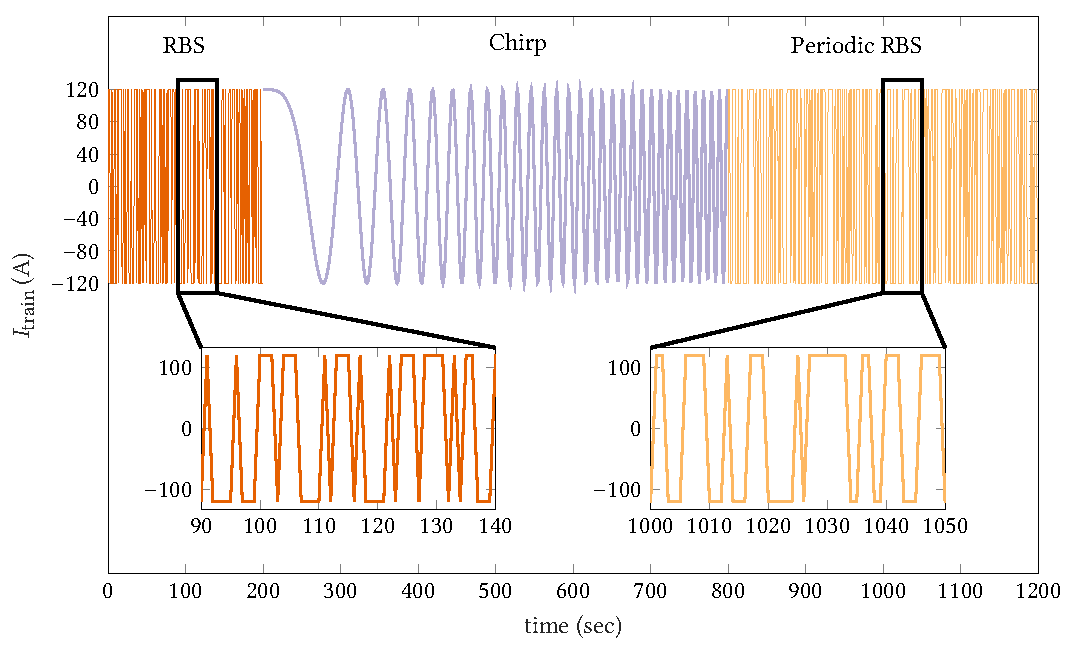
\includegraphics{4/figures/sysid_train_input.pdf}
    \captionsetup{singlelinecheck=off}
    \caption[Input current profile used as the training set for system
    identification]{Input current profile used as the training set for system
    identification. The sequence consists of
    \begin{enumerate*}[label=\emph{\alph*})] \item a \glsfmtlong{rbs}, \item a
        chirp or swept cosine signal (0--\SI{100}{\milli\hertz}), and \item a periodic \glsfmtlong{rbs} \end{enumerate*} thereby
covering both low and high frequency spectra while incorporating the potential
to excite any periodic modes in the system to be identified.}
    \label{fig:sysidtrainingcurrent}
\end{figure}

% Testing input current

For  the  purposes  of  identification,  the \gls{p2d}  model  is  used  as  the
input.  First, the  current profile  from  the training  set is  applied to  the
\gls{p2d} model. Its  simulation results, in particular,  the numerically solved
concentration values  at each spatially  discretised node  in each of  the three
regions per  time-step is then integrated  over the thickness of  the respective
regions  and multiplied  with their  respective porosities.  Thus the  number of
moles of \ch{Li^+}  per unit area in each of  the three regions $Q_{\text{e,}j}$
are obtained. Only  the quantities $Q_\text{e,n}$ and  $Q_\text{e,p}$ are chosen
as the outputs for system identification and a transfer function model is fitted
as per the evaluation procedure discussed in~\cref{subsubsec:actualsysid}.

As with  any classical  curve fitting  (numerical regression)  procedure, system
identification is also  prone to overfitting the training data.  In general, the
`best' transfer  function that identifies the  given system is the  lowest order
model that  can not  only minimize  the training error,  but also  minimizes the
error  on  a  previously  unseen  validation  dataset.  In  the  absence  of  an
independent validation dataset, the training error can be made arbitrarily small
by increasing  the number  of poles  and zeros of  the transfer  function models
without any  bounds. However, such a  model shall not have  truly identified the
dynamics of  the system  and shall  not generalise  well to  real-world datasets
outside  the training  realm. Hence,  having an  independent validation  current
profile for the task at hand is of paramount importance.

For the system identification task at  hand, the characteristic waveforms of the
validation profile were deliberately conjured to be differ vastly from that used
in training the model. The  validation profile consists of the following
sequence
\begin{enumerate}
    \item Periodic \gls{rgs} with 4 periods of \SI{200}{\second} each\quad (0--\SI{799}{\second})
    \item \gls{prbs} for emulating white noise, \ie{} with a flat power spectra
        across the frequency spectrum\quad (800--\SI{999}{\second})
    \item Multi-sine signal \ie{} a signal consisting of sinusoids at
        various fundamental frequencies added together\quad (1000--\SI{1199}{\second})
\end{enumerate}

Overall,  the validation  profile has  been designed  to cover  a wide  range of
frequencies  akin to  the  training  profile, but  differing  completely in  its
time-domain appearance.  The specific  validation current  profile used  in this
system identification is shown in~\cref{fig:sysidvalidationcurrent}.

\begin{figure}[!htb]
    \centering
    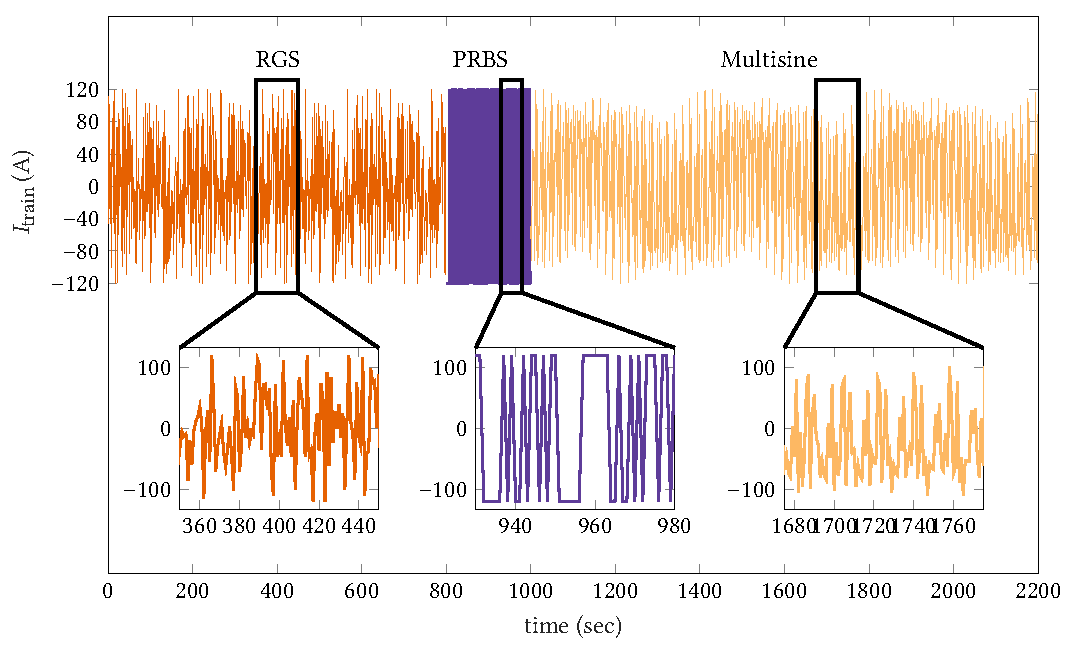
\includegraphics{4/figures/sysid_validation_input.pdf}
    \captionsetup{singlelinecheck=off}
    \caption[Input current profile used as the validation set for system
    identification]{Input current profile used as the validation set for system
        identification. The sequence consists of
        \begin{enumerate*}[label=\emph{\alph*})]
            \item a \glsfmtlong{rgs},
            \item a \glsfmtlong{prbs}, and
            \item a multisine waveform
        \end{enumerate*}.
        The overall sequence  is intended to emulate the flat  power spectrum of
        white noise (with the \glsfmtshort{prbs}) and excite any poles and zeros
        within  3$\sigma$ spread  of the  \glsfmtshort{rgs} mean.  The multisine
        signal is  swept is composed  of sinusoids with  fundamental frequencies
        from \SI{100}{\milli\hertz}  up to the Nyquist  frequency. Its amplitude
        variation  across the  frequency spectrum  increases the  probability to
        capture the  system's modes that  were possibly missed by  the preceding
        two waveforms.
    }%
    \label{fig:sysidvalidationcurrent}
\end{figure}

MATLAB  code that  can be  used to  generate the  training and  validation input
profiles is shown in~\cref{codesnippet:trainvalidsysidinput}.

\begin{listing}[!htbp]
\begin{minted}[mathescape,autogobble,bgcolor=mintedbg,escapeinside=||,texcomments=true]{matlab}
% Needs matlab's system identification toolbox
clear; close all; clc; format short g;
warning('off','Ident:dataprocess:idinput7'); % suppress sysid warnings
I_1C  = 60; % Amps
range = 2*[-I_1C I_1C]; % peak-peak swing is $\pm 2\text{C}=\SI{40}{\ampere}$
NumCh = 1; % no of channels (used by sysid toolbox for multichannel id)
Ts    = 1; % sampling interval

%% Random Binary Input Signal (RBS)
N  = 200; % samples per quantum of each waveform
u1 = idinput(N,'rbs',[],range); % 'idinput' from sysid toolbox
%% Chirp Signal (swept cosine)
t_chirp_start = 0;
t_chirp_end   = 3*N*Ts; %
t             = linspace(t_chirp_start,t_chirp_end,3*N);
f0            = 0;
f1            = 1e-1; % $f_1 = \SI{100}{\milli\hertz}$ is the max chirp frequency
u2            = max(range)*chirp(t,f0,t(end),f1)';
%% Periodic Random Binary Input Signal (Periodic RBS)
bin_seq_Period   = N; % seconds
bin_seq_Period_N = ceil(bin_seq_Period/Ts); % samples
bin_NumPeriod    = 2;
u3 = idinput([bin_seq_Period_N,NumCh,bin_NumPeriod],'rbs',[],range);
%% Random Guassian Signal (RGS)
rgs_Period         = N; % seconds
rgs_Period_samples = ceil(rgs_Period/Ts);
rgs_NumPeriod      = 4;
u4 = idinput([rgs_Period_samples,NumCh,rgs_NumPeriod],'rgs',[],range/2);
%% PseudoRandom Binary Signal (PRBS)
prbs_Period         = N; % seconds
prbs_Period_samples = ceil(prbs_Period/Ts);
u5                  = idinput(N,'prbs',[],range);
%% Multisine signal (sum of sines)
samples_per_Period = 2*N;
NumPeriod          = 3;
[u6,freq] = idinput([samples_per_Period 1 NumPeriod],'sine',[],range);

%% Split into training and validation data sets
I_load_train    = [u1;u2;u3];
I_load_validate = [u4;u5;u6];
\end{minted}
\caption{Generation of training and validation input current profiles in MATLAB}
\label{codesnippet:trainvalidsysidinput}
\end{listing}

% Linearity and time-invariance

The      transfer     function      identification     techniques      mentioned
in~\cref{subsubsec:introblackboxsysid}   are  applicable  only   for   \gls{lti}
systems.  At the  first glance,  this seems  overly restrictive  for the  system
at  hand.  A lithium  ion  battery,  when  considered  as a  single  macroscopic
entity,  exhibits non-linear  characteristics,  particularly due  to the  strong
non-linearities in
\begin{enumerate*}[label=\emph{\alph*})]
    \item the Butler-Volmer reaction kinetics (see~\cref{eq:butlervolmer}), and
    \item the \glspl{ocp} of the two electrodes (see~\cref{eq:lcoUocpPos} and~\cref{eq:lcoUocpPos}).
\end{enumerate*}
However, since we are dealing with a much narrower scope \ie{} the systems under
consideration  are just  the two  sub-system entities  (one per  electrode) that
transform the  applied current at  a particular  time-step to the  overall moles
per  unit area  of  \ch{Li^+}  ions in  the  corresponding  electrode region  of
the  electrolyte at  that  same  instant. Therefore,  it  is  the linearity  and
time-invariance of these \emph{subsystems} that must be investigated.

A  test  for time-invariance  is  prescribed  in  the  lecture notes  on  system
identification by  Plett~\cite{PlettECE5560_02}. The steps involved  therein are
reproduced here after  being suitably adapted to the notation  of the subsystems
at hand.
\begin{enumerate}
    \item Apply input $u_1(t) = I(t)$ to the system and measure the outputs $\widetilde{Q}_{\text{e,n}_1}(t)$ and $\widetilde{Q}_{\text{e,p}_1}(t)$.
    \item Apply a delayed version of the input by $\tau$ seconds \ie{} $u_2(t) = I(t-\tau)$ to the system and measure the outputs
        $\widetilde{Q}_{\text{e,n}_2}(t)$ and $\widetilde{Q}_{\text{e,n}_2}(t)$.
    \item If $\widetilde{Q}_{\text{e,n}_2}(t)$ = $\widetilde{Q}_{\text{e,n}_1}(t-\tau)$ and $\widetilde{Q}_{\text{e,p}_2}(t)$ = $\widetilde{Q}_{\text{e,p}_1}(t-\tau)$ for all possible delays $\tau$ as well as for choice of input signals $I(t)$, then the systems are time-invariant.
\end{enumerate}

For  the  systems   at  hand,  it  is  not  strictly   required  to  apply  this
prescriptive  test.  Unless a  fundamental  change  in the  underlying  reaction
phenomena/chemistry  occur that  alter the  performance over  time, systems  are
treated  as time-invariant.  Factors  that induce  time-dependent  shift in  the
behaviour of lithium ion batteries  are degradation phenomena such as thickening
of \gls{sei} layer  on the electrodes, dendrite growth or  mechanical fatigue in
electrodes  which in-turn  affect electrolytic  diffusion and  conductivity. Yet
another cause  of time-dependent  behavioural change is  the drift  in parameter
values. However, these  phenomena are typically one or mode  orders of magnitude
slower than  the \gls{p2d} dynamics\fxnote{citation needed}.  This separation of
time-scales  imply  that in  practice,  they  can  be decoupled  and  therefore,
separate  models can  be  identified  for the  faster  and  slower processes.  A
suitable model-blending approach  can then be considered to arrive  at cover all
processes across time-scales. Although the  concepts developed here for the fast
electrolyte dynamics can be suitably adapted to such slow phenomena, their study
falls outside  the scope of this  thesis and is  left as an exercise  for future
work.  Thus,  the overall  battery  system,  and  hence  by extension,  the  two
subsystems considered are deemed to  be time-invariant. However, in the interest
of  completeness, this  author  systematically applied  the aforementioned  test
procedure  with every  combination arising  from  the choice  of ten  time-delay
values and the following five current profiles ---
\begin{enumerate*}[label=\emph{\alph*})]
    \item constant current 1C discharge,
    \item constant current 3C discharge,
    \item constant current 1C charge,
    \item \gls{udds} input profile with peak amplitude of 3C,
    \item training profile used in system identification (see~\cref{fig:sysidtrainingcurrent}), and
    \item validation profile used in system identification (see~\cref{fig:sysidvalidationingcurrent}).
\end{enumerate*}
All tests successfully  passed, with the delayed version of  all of the original
output signals accurately matching their  responses to the corresponding delayed
input (down to  machine precision), thereby confirming the  time-variance of the
subsystems considered in the system identification problem.


In the analyses of linearity of systems, it is a recommended practice to de-bias
the output and input quantities about their mean operating conditions. The input
signal in this case, is the applied load current $I(t)$. This signal can be both
positive (during  discharge) and negative  (during charge). Although  in typical
drive-cycles, there is  a net discharge, the specific value  of the mean applied
current does  not generalise  well across drivecycles.  Furthermore, drivecycles
are merely representative  profiles and certainly, in  real-world operation, the
cell needs to be  treated as being equally probable for  being subjected to both
charging and discharging currents. Hence, the  mean of the input signal is taken
as zero, eliminating any de-biasing requirements.

For the output  signals though, there is  clearly a bias. The  overall number of
moles of  \ch{Li^+} in  any region  cannot be  physically negative.  Even though
under  high C-rates,  ion  depletion  at localised  spatial  locations (such  as
the  current collectors)  is certainly  possible,  the entire  thickness of  any
region  cannot be  devoid of  ions at  any point  in time  since the  cell shall
instantaneously  cease  to  work  further. Thus,  for  a  typical  well-designed
cell  operating within  the manufacturer  prescribed C-rate  limits, the  output
signals  under consideration  operate  in  a small  window  about their  initial
values. In  the author's  simulations, even  at $\pm$5C,  the overall  number of
moles  of \ch{Li^+}  in  any cell  region  exhibited a  maximum  change of  less
than  \SI{15}{\percent}  from its  initial  value.  Thus, the  de-biased  output
variables  for  system  identification, $\widetilde{Q}_{\text{e}_j}(t)$  can  be
obtained  by subtracting  their  respective  initial values  $Q_{\text{e,}j}(0)$
(see~\cref{eq:Qeninit} and~\cref{eq:Qepinit}) from $Q_{\text{e,}j}(t)$.
\begin{align}
    \widetilde{Q}_\text{e,n}(t) &= {Q}_\text{e,n}(t) - {Q}_\text{e,n}(0) \\
    \widetilde{Q}_\text{e,p}(t) &= {Q}_\text{e,p}(t) - {Q}_\text{e,p}(0)
\end{align}
which   implies   that   the   transfer  functions   to   be   identified   have
to   be   modified    to   be   $\frac{\widetilde{Q}_\text{e,n}(s)}{I(s)}$   and
$\frac{\widetilde{Q}_\text{e,p}(s)}{I(s)}$ respectively.

\subsubsection*{actual procedure briefly}\label{subsubsec:actualsysid}

% Assumed transfer function model. Test results within the model itself
% Test results for electrolyte ce (subsection)
% test results for full system (final section)


% mention in introduction where code snippets are given
